\documentclass[exos]{nsi}
\titre{Classes \texttt{NSI}}
\classe{2023-06}
\begin{document}
\maketitle

\section{Classes et options}
4 classes sont disponibles :
\begin{itemize}
    \item \texttt{nsibook}, qui hérite de la classe \texttt{book} ;
    \item \texttt{nsieval}, qui hérite de la classe \texttt{article} ;
    \item \texttt{nsiarticle}, qui hérite de la classe \texttt{article} ;
    \item \texttt{nsiexo}, qui hérite également de la classe \texttt{article} ;
\end{itemize}
Ainsi les options disponibles pour \texttt{book} ou pour les autres classes le restent.

\begin{minted}[bgcolor=yellow!10!white]{latex}
\documentclass[12pt,a4paper]{nsibook} % ou 10pt, ou 11pt
    \begin{document}
        ...
    \end{document}
\end{minted}


\section{Environnements}
\subsection*{Définition}
\begin{minted}[bgcolor=yellow!10!white]{latex}
    \begin{definition}[ : précision]
        contenu
    \end{definition} 
\end{minted}
\begin{definition}[ : précision]
    contenu
\end{definition}
\subsection*{Exemple}
\begin{minted}[bgcolor=yellow!10!white]{latex}
    \begin{exemple}[ : précision]
        contenu
    \end{exemple} 
\end{minted}
\begin{exemple}[ : précision]
    contenu
\end{exemple}
\subsection*{Propriété}
\begin{minted}[bgcolor=yellow!10!white]{latex}
    \begin{propriete}[ : précision]
        contenu
    \end{propriete} 
\end{minted}
\begin{propriete}[ : précision]
    contenu
\end{propriete}
\subsection*{Notation}
\begin{minted}[bgcolor=yellow!10!white]{latex}
    \begin{notation}[ : précision]
        contenu
    \end{notation} 
\end{minted}
\begin{notation}[ : précision]
    contenu
\end{notation}
\subsection*{Méthode}
\begin{minted}[bgcolor=yellow!10!white]{latex}
    \begin{methode}[ : précision]
        contenu
    \end{methode} 
\end{minted}
\begin{methode}[ : précision]
    contenu
\end{methode}
\subsection*{Remarque}
\begin{minted}[bgcolor=yellow!10!white]{latex}
    \begin{remarque}[ : précision]
        contenu
    \end{remarque} 
\end{minted}
\begin{remarque}[ : précision]
    contenu
\end{remarque}
\subsection*{À retenir}
\begin{minted}[bgcolor=yellow!10!white]{latex}
    \begin{aretenir}[ : précision]
        contenu
    \end{aretenir} 
\end{minted}
\begin{aretenir}[ : précision]
    contenu
\end{aretenir}

\section{Pour le code}
\begin{minted}[bgcolor=yellow!10!white]{latex}
\begin{pyc}
    \begin{minted}{python}
        def f(x: float) -> float:
            return 0.5 * x ** 2
    end{minted} % avec un \ devant
end{pyc}% avec un \ devant
\end{minted}
\begin{pyc}
    \begin{minted}{python}
        def f(x: float) -> float:
            return 0.5 * x ** 2
    \end{minted}
\end{pyc}

\begin{minted}[bgcolor=yellow!10!white]{latex}
    Je veux vous parler de la fonction \mintinline{python}{print} de \textsc{Python}. 
\end{minted}
Je veux vous parler de la fonction \mintinline{python}{print} de \textsc{Python}.


\subsection*{Encadré coloré custom}

\begin{minted}[bgcolor=yellow!10!white]{latex}
    \begin{encadrecolore}{Titre customisé de la couleur désirée}{UGLiDarkBlue}
        contenu
    \end{encadrecolore}
\end{minted}
\begin{encadrecolore}{Titre customisé de la couleur désirée}{UGLiDarkBlue}
    contenu
\end{encadrecolore}

\section{Environnements énumératifs}
\subsection*{Liste ordonnée}
\begin{minted}[bgcolor=yellow!10!white]{latex}
\begin{enumerate}
    \item truc ;
    \item machin ;
    \item bidule.
\end{enumerate}
\end{minted}
\begin{enumerate}
    \item truc ;
    \item machin ;
    \item bidule
\end{enumerate}

\subsection*{Liste non ordonnée}
\begin{minted}[bgcolor=yellow!10!white]{latex}
\begin{itemize}
    \item truc ;
    \item machin ;
    \item bidule.
\end{itemize}
\end{minted}

\begin{itemize}
    \item truc ;
    \item machin ;
    \item bidule.
\end{itemize}

\subsection*{QCM}
\begin{minted}[bgcolor=yellow!10!white]{latex}
Une question à choix multiples
\begin{qcm}
    \item Réponse 1
    \item Réponse 2
    \item Réponse 3
\end{qcm}
\end{minted}
Une question à choix multiples
    \begin{qcm}
        \item Réponse 1
        \item Réponse 2
        \item Réponse 3
\end{qcm}

\section{Couleurs}
\begin{minted}[bgcolor=yellow!10!white]{latex}
    \color{UGLiPurple} UGLiPurple \\
    \color{UGLiRed} UGLiRed \\
    \color{UGLiOrange} UGLiOrange \\
    \color{UGLiYellow} UGLiYellow \\
    \color{UGLiGreen} UGLiGreen \\
    \color{UGLiDarkGreen} UGLiDarkGreen \\
    \color{UGLiBlue} UGLiBlue \\
    \color{UGLiDarkBlue} UGLiDarkBlue 
\end{minted}
\color{UGLiPurple} UGLiPurple \\
\color{UGLiRed} UGLiRed \\
\color{UGLiOrange} UGLiOrange \\
\color{UGLiYellow} UGLiYellow \\
\color{UGLiGreen} UGLiGreen \\
\color{UGLiDarkGreen} UGLiDarkGreen \\
\color{UGLiBlue} UGLiBlue \\
\color{UGLiDarkBlue} UGLiDarkBlue \color{black}

\section{Tables}

\begin{minted}[bgcolor=yellow!10!white]{latex}
    \tabularstyled
    \begin{tabular}{c|c|c}
        \rowcolor{UGLiOrange}
        \ths Colonne 1 & \ths Colonne 2 & \ths Colonne 3 \\
        Valeur 1 & Valeur 2 & Valeur 3 \\
        Valeur 4 & Valeur 5 & Valeur 6 \\
        Valeur 7 & Valeur 8 & Valeur 9 \\
        Valeur 10 & Valeur 11 & Valeur 12 \\
        Valeur 13 & Valeur 14 & Valeur 15 \\
    \end{tabular}    
\end{minted}
\tabularstyled
\begin{tabular}{c|c|c}
    \rowcolor{UGLiOrange}
    \ths Colonne 1 & \ths Colonne 2 & \ths Colonne 3 \\
    Valeur 1       & Valeur 2       & Valeur 3       \\
    Valeur 4       & Valeur 5       & Valeur 6       \\
    Valeur 7       & Valeur 8       & Valeur 9       \\
    Valeur 10      & Valeur 11      & Valeur 12      \\
    Valeur 13      & Valeur 14      & Valeur 15      \\
\end{tabular}

\begin{minted}[bgcolor=yellow!10!white]{latex}
    \tabularstyled[UGLiPurple]
    \begin{tabular}{c|c|c}
        \rowcolor{UGLiPurple}
        \ths Colonne 1 & \ths Colonne 2 & \ths Colonne 3 \\
        Valeur 1 & Valeur 2 & Valeur 3 \\
        Valeur 4 & Valeur 5 & Valeur 6 \\
        Valeur 7 & Valeur 8 & Valeur 9 \\
        Valeur 10 & Valeur 11 & Valeur 12 \\
        Valeur 13 & Valeur 14 & Valeur 15 \\
    \end{tabular}    
\end{minted}
\tabularstyled[UGLiPurple]
\begin{tabular}{c|c|c}
    \rowcolor{UGLiPurple}
    \ths Colonne 1 & \ths Colonne 2 & \ths Colonne 3 \\
    Valeur 1       & Valeur 2       & Valeur 3       \\
    Valeur 4       & Valeur 5       & Valeur 6       \\
    Valeur 7       & Valeur 8       & Valeur 9       \\
    Valeur 10      & Valeur 11      & Valeur 12      \\
    Valeur 13      & Valeur 14      & Valeur 15      \\
\end{tabular}
\begin{minted}[bgcolor=yellow!10!white]{latex}
    \tabulardefault
    \begin{tabular}{|c|c|c|}
        \hline
         Colonne 1 & Colonne 2 & Colonne 3 \\
        \hline
        Valeur 1 & Valeur 2 & Valeur 3 \\
        Valeur 4 & Valeur 5 & Valeur 6 \\
        Valeur 7 & Valeur 8 & Valeur 9 \\
        Valeur 10 & Valeur 11 & Valeur 12 \\
        Valeur 13 & Valeur 14 & Valeur 15 \\
        \hline
    \end{tabular}
\end{minted}
\tabulardefault
\begin{tabular}{|c|c|c|}
    \hline
    Colonne 1 & Colonne 2 & Colonne 3 \\
    \hline
    Valeur 1  & Valeur 2  & Valeur 3  \\
    Valeur 4  & Valeur 5  & Valeur 6  \\
    Valeur 7  & Valeur 8  & Valeur 9  \\
    Valeur 10 & Valeur 11 & Valeur 12 \\
    Valeur 13 & Valeur 14 & Valeur 15 \\
    \hline
\end{tabular}

\section{Mise en page}

\begin{minted}[bgcolor=yellow!10!white]{latex}
    Du texte avant.\\
    \floatpictureleft{0.3}{iris.png}{
        Une image à gauche avec du texte à droite. En général on s'arrange pour que le premier paramètre, qui est la fraction de la largeur de la ligne occupée par l'image et la quantité de texte à droite soient en harmonie sinon voici ce que cela donne.
        }\par\medskip
    Du texte après.
\end{minted}
Du texte avant.\\
\floatpictureleft{0.3}{iris.png}{ Une image à gauche avec du texte à droite. En général on s'arrange pour que le premier paramètre, qui est la fraction de la largeur de la ligne occupée par l'image et la quantité de texte à droite soient en harmonie sinon voici ce que cela donne.}\par\medskip
Du texte après.

\begin{minted}[bgcolor=yellow!10!white]{latex}
Du texte avant, qui peut prendre toute la ligne ou pas.\\
\floatpictureleft{0.15}{iris.png}{
    Une image à gauche avec du texte à droite. En général on s'arrange pour que le premier paramètre, qui est la fraction de la largeur de la ligne occupée par l'image et la quantité de texte à droite soient en harmonie sinon on a vu ce que ça donne. Ce n'est pas catastrophique et cela peut même être désiré, mais en s'y prenant bien, voici à quoi on arrive. Ce n'est pas parfait mais je n'ai pas trouvé mieux !
    }\par\medskip
Du texte après, qui peut prendre toute la ligne ou pas.
\end{minted}
Du texte avant, qui peut prendre toute la ligne ou pas.\\
\floatpictureleft{0.15}{iris.png}{ Une image à gauche avec du texte à droite. En général on s'arrange pour que le premier paramètre, qui est la fraction de la largeur de la ligne occupée par l'image et la quantité de texte à droite soient en harmonie sinon on a vu ce que ça donne. Ce n'est pas catastrophique et cela peut même être désiré, mais en s'y prenant bien, voici à quoi on arrive. Ce n'est pas parfait mais je n'ai pas trouvé mieux ! }\par\medskip
Du texte après, qui peut prendre toute la ligne ou pas.\\

\begin{minted}[bgcolor=yellow!10!white]{latex}
\floatpictureleftcaption{0.15}{iris.png}{Quel belle fleur !}{ 
    Une image \textit{légendée} à gauche avec du texte à droite : observez la légende en dessous de l'image.\\
    En général on s'arrange pour que le premier paramètre, qui est la fraction de la largeur de la ligne occupée par l'image et la quantité de texte à droite soient en harmonie sinon on a vu ce que ça donne.\\
    Ce n'est pas catastrophique et cela peut même être désiré, mais en s'y prenant bien, voici à quoi on arrive. Ce n'est pas parfait mais je n'ai pas trouvé mieux ! }\par\medskip
Du texte après, qui peut prendre toute la ligne ou pas.
\end{minted}
\floatpictureleftcaption{0.15}{iris.png}{Quel belle fleur !}{
    Une image \textit{légendée} à gauche avec du texte à droite : observez la légende en dessous de l'image.\\
    En général on s'arrange pour que le premier paramètre, qui est la fraction de la largeur de la ligne occupée par l'image et la quantité de texte à droite soient en harmonie sinon on a vu ce que ça donne.\\
    Ce n'est pas catastrophique et cela peut même être désiré, mais en s'y prenant bien, voici à quoi on arrive. Ce n'est pas parfait mais je n'ai pas trouvé mieux ! }\par\medskip
Du texte après, qui peut prendre toute la ligne ou pas.

\section{Tableaux de variations}
\begin{minted}[bgcolor=yellow!10!white]{latex}
    \begin{center}
        \begin{tikzpicture}
            \tkzTabInit[color,lgt=2,espcl=2]
            {$x$ /.7 ,$f'(x)$ /.7,$f$ /1.4}
            {$-\infty$, -1 ,5, $+\infty$ }
            \tkzTabLine{,+ , z, -,z,+,}
            \tkzTabVar{-/,+/,-/,+/}
        \end{tikzpicture}
    \end{center}   
\end{minted}

\begin{center}
    \begin{tikzpicture}
        \tkzTabInit[color,lgt=2,espcl=2]
        {$x$ /.7 ,$f'(x)$ /.7,$f$ /1.4}
        {$-\infty$, -1 ,5, $+\infty$ }
        \tkzTabLine{,+ , z, -,z,+,}
        \tkzTabVar{-/,+/,-/,+/}
    \end{tikzpicture}
\end{center}

\section{Courbes représentatives}
\begin{minted}[bgcolor=yellow!10!white]{latex}
\begin{center}
    \def\xmin{-1} \def\ymin{-1}\def\xmax{3}\def\ymax{2}
    \def\F{\x-(\x)^(.5)}
    \begin{tikzpicture}[scale=2]
        \clip (\xmin,\ymin) rectangle (\xmax,\ymax);
        \draw[fill = white] (\xmin,\ymin) rectangle (\xmax,\ymax);
        \reperev{\xmin}{\ymin}{\xmax}{\ymax}
        \draw[thick,domain=0:\xmax,samples=1000,UGLiOrange,variable=\x] plot ({\x},{\F});    
        \point{1}{1}{A} 
    \end{tikzpicture}
\end{center}
\end{minted}
\begin{center}
    \def\xmin{-1} \def\ymin{-1}\def\xmax{3}\def\ymax{2}
    \def\F{\x-(\x)^(.5)}
    \begin{tikzpicture}[scale=2]
        \clip (\xmin,\ymin) rectangle (\xmax,\ymax);
        \draw[fill = white] (\xmin,\ymin) rectangle (\xmax,\ymax);
        \reperev{\xmin}{\ymin}{\xmax}{\ymax}
        \draw[thick,domain=0:\xmax,samples=1000,UGLiOrange,variable=\x] plot ({\x},{\F});    
        \point{1}{1}{A} 
    \end{tikzpicture}
\end{center}

\section{Arbre de probabilités}

\begin{minted}[bgcolor=yellow!10!white]{latex}
\def\abun{A}
\def\alun{0,1}

\def\abdeux{$\barmaj{A}$}
\def\aldeux{\ldots}

\def\abtrois{$A\cap B$}
\def\altrois{$p_A(B)$}

\def\abquatre{$A\cap\barmaj{B}$}
\def\alquatre{0,7}

\def\abcinq{$\barmaj{A}\cap B$}
\def\alcinq{0,4}

\def\absix{$\barmaj{A}\cap\barmaj{B}$}
\def\alsix{\ldots}

\begin{center}
    \arbreproba
\end{center}
\end{minted}
\def\abun{A}
\def\alun{0,1}

\def\abdeux{$\barmaj{A}$}
\def\aldeux{\ldots}

\def\abtrois{$A\cap B$}
\def\altrois{$p_A(B)$}

\def\abquatre{$A\cap\barmaj{B}$}
\def\alquatre{0,7}

\def\abcinq{$\barmaj{A}\cap B$}
\def\alcinq{0,4}

\def\absix{$\barmaj{A}\cap\barmaj{B}$}
\def\alsix{\ldots}

\begin{center}
    \arbreproba
\end{center}

\end{document}
